\documentclass[1p]{elsarticle_modified}
%\bibliographystyle{elsarticle-num}

%\usepackage[colorlinks]{hyperref}
%\usepackage{abbrmath_seonhwa} %\Abb, \Ascr, \Acal ,\Abf, \Afrak
\usepackage{amsfonts}
\usepackage{amssymb}
\usepackage{amsmath}
\usepackage{amsthm}
\usepackage{scalefnt}
\usepackage{amsbsy}
\usepackage{kotex}
\usepackage{caption}
\usepackage{subfig}
\usepackage{color}
\usepackage{graphicx}
\usepackage{xcolor} %% white, black, red, green, blue, cyan, magenta, yellow
\usepackage{float}
\usepackage{setspace}
\usepackage{hyperref}

\usepackage{tikz}
\usetikzlibrary{arrows}

\usepackage{multirow}
\usepackage{array} % fixed length table
\usepackage{hhline}

%%%%%%%%%%%%%%%%%%%%%
\makeatletter
\renewcommand*\env@matrix[1][\arraystretch]{%
	\edef\arraystretch{#1}%
	\hskip -\arraycolsep
	\let\@ifnextchar\new@ifnextchar
	\array{*\c@MaxMatrixCols c}}
\makeatother %https://tex.stackexchange.com/questions/14071/how-can-i-increase-the-line-spacing-in-a-matrix
%%%%%%%%%%%%%%%

\usepackage[normalem]{ulem}

\newcommand{\msout}[1]{\ifmmode\text{\sout{\ensuremath{#1}}}\else\sout{#1}\fi}
%SOURCE: \msout is \stkout macro in https://tex.stackexchange.com/questions/20609/strikeout-in-math-mode

\newcommand{\cancel}[1]{
	\ifmmode
	{\color{red}\msout{#1}}
	\else
	{\color{red}\sout{#1}}
	\fi
}

\newcommand{\add}[1]{
	{\color{blue}\uwave{#1}}
}

\newcommand{\replace}[2]{
	\ifmmode
	{\color{red}\msout{#1}}{\color{blue}\uwave{#2}}
	\else
	{\color{red}\sout{#1}}{\color{blue}\uwave{#2}}
	\fi
}

\newcommand{\Sol}{\mathcal{S}} %segment
\newcommand{\D}{D} %diagram
\newcommand{\A}{\mathcal{A}} %arc


%%%%%%%%%%%%%%%%%%%%%%%%%%%%%5 test

\def\sl{\operatorname{\textup{SL}}(2,\Cbb)}
\def\psl{\operatorname{\textup{PSL}}(2,\Cbb)}
\def\quan{\mkern 1mu \triangleright \mkern 1mu}

\theoremstyle{definition}
\newtheorem{thm}{Theorem}[section]
\newtheorem{prop}[thm]{Proposition}
\newtheorem{lem}[thm]{Lemma}
\newtheorem{ques}[thm]{Question}
\newtheorem{cor}[thm]{Corollary}
\newtheorem{defn}[thm]{Definition}
\newtheorem{exam}[thm]{Example}
\newtheorem{rmk}[thm]{Remark}
\newtheorem{alg}[thm]{Algorithm}

\newcommand{\I}{\sqrt{-1}}
\begin{document}

%\begin{frontmatter}
%
%\title{Boundary parabolic representations of knots up to 8 crossings}
%
%%% Group authors per affiliation:
%\author{Yunhi Cho} 
%\address{Department of Mathematics, University of Seoul, Seoul, Korea}
%\ead{yhcho@uos.ac.kr}
%
%
%\author{Seonhwa Kim} %\fnref{s_kim}}
%\address{Center for Geometry and Physics, Institute for Basic Science, Pohang, 37673, Korea}
%\ead{ryeona17@ibs.re.kr}
%
%\author{Hyuk Kim}
%\address{Department of Mathematical Sciences, Seoul National University, Seoul 08826, Korea}
%\ead{hyukkim@snu.ac.kr}
%
%\author{Seokbeom Yoon}
%\address{Department of Mathematical Sciences, Seoul National University, Seoul, 08826,  Korea}
%\ead{sbyoon15@snu.ac.kr}
%
%\begin{abstract}
%We find all boundary parabolic representation of knots up to 8 crossings.
%
%\end{abstract}
%\begin{keyword}
%    \MSC[2010] 57M25 
%\end{keyword}
%
%\end{frontmatter}

%\linenumbers
%\tableofcontents
%
\newcommand\colored[1]{\textcolor{white}{\rule[-0.35ex]{0.8em}{1.4ex}}\kern-0.8em\color{red} #1}%
%\newcommand\colored[1]{\textcolor{white}{ #1}\kern-2.17ex	\textcolor{white}{ #1}\kern-1.81ex	\textcolor{white}{ #1}\kern-2.15ex\color{red}#1	}

{\Large $\underline{12a_{0279}~(K12a_{0279})}$}

\setlength{\tabcolsep}{10pt}
\renewcommand{\arraystretch}{1.6}
\vspace{1cm}\begin{tabular}{m{100pt}>{\centering\arraybackslash}m{274pt}}
\multirow{5}{120pt}{
	\centering
	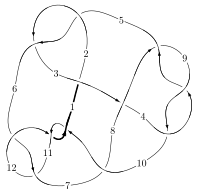
\includegraphics[width=112pt]{../../../GIT/diagram.site/Diagrams/png/1080_12a_0279.png}\\
\ \ \ A knot diagram\footnotemark}&
\allowdisplaybreaks
\textbf{Linearized knot diagam} \\
\cline{2-2}
 &
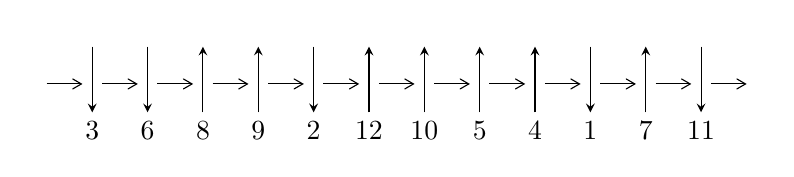
\begin{tikzpicture}[x=20pt, y=17pt]
	% nodes
	\node (C0) at (0, 0) {};
	\node (C1) at (1, 0) {};
	\node (C1U) at (1, +1) {};
	\node (C1D) at (1, -1) {3};

	\node (C2) at (2, 0) {};
	\node (C2U) at (2, +1) {};
	\node (C2D) at (2, -1) {6};

	\node (C3) at (3, 0) {};
	\node (C3U) at (3, +1) {};
	\node (C3D) at (3, -1) {8};

	\node (C4) at (4, 0) {};
	\node (C4U) at (4, +1) {};
	\node (C4D) at (4, -1) {9};

	\node (C5) at (5, 0) {};
	\node (C5U) at (5, +1) {};
	\node (C5D) at (5, -1) {2};

	\node (C6) at (6, 0) {};
	\node (C6U) at (6, +1) {};
	\node (C6D) at (6, -1) {12};

	\node (C7) at (7, 0) {};
	\node (C7U) at (7, +1) {};
	\node (C7D) at (7, -1) {10};

	\node (C8) at (8, 0) {};
	\node (C8U) at (8, +1) {};
	\node (C8D) at (8, -1) {5};

	\node (C9) at (9, 0) {};
	\node (C9U) at (9, +1) {};
	\node (C9D) at (9, -1) {4};

	\node (C10) at (10, 0) {};
	\node (C10U) at (10, +1) {};
	\node (C10D) at (10, -1) {1};

	\node (C11) at (11, 0) {};
	\node (C11U) at (11, +1) {};
	\node (C11D) at (11, -1) {7};

	\node (C12) at (12, 0) {};
	\node (C12U) at (12, +1) {};
	\node (C12D) at (12, -1) {11};
	\node (C13) at (13, 0) {};

	% arrows
	\draw[->,>={angle 60}]
	(C0) edge (C1) (C1) edge (C2) (C2) edge (C3) (C3) edge (C4) (C4) edge (C5) (C5) edge (C6) (C6) edge (C7) (C7) edge (C8) (C8) edge (C9) (C9) edge (C10) (C10) edge (C11) (C11) edge (C12) (C12) edge (C13) ;	\draw[->,>=stealth]
	(C1U) edge (C1D) (C2U) edge (C2D) (C3D) edge (C3U) (C4D) edge (C4U) (C5U) edge (C5D) (C6D) edge (C6U) (C7D) edge (C7U) (C8D) edge (C8U) (C9D) edge (C9U) (C10U) edge (C10D) (C11D) edge (C11U) (C12U) edge (C12D) ;
	\end{tikzpicture} \\
\hhline{~~} \\& 
\textbf{Solving Sequence} \\ \cline{2-2} 
 &
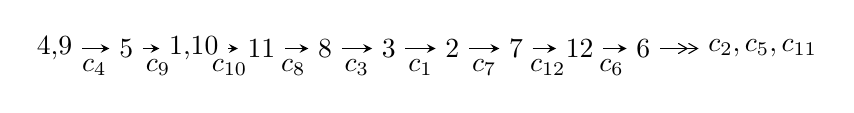
\begin{tikzpicture}[x=23pt, y=7pt]
	% node
	\node (A0) at (-1/8, 0) {4,9};
	\node (A1) at (1, 0) {5};
	\node (A2) at (33/16, 0) {1,10};
	\node (A3) at (25/8, 0) {11};
	\node (A4) at (33/8, 0) {8};
	\node (A5) at (41/8, 0) {3};
	\node (A6) at (49/8, 0) {2};
	\node (A7) at (57/8, 0) {7};
	\node (A8) at (65/8, 0) {12};
	\node (A9) at (73/8, 0) {6};
	\node (C1) at (1/2, -1) {$c_{4}$};
	\node (C2) at (3/2, -1) {$c_{9}$};
	\node (C3) at (21/8, -1) {$c_{10}$};
	\node (C4) at (29/8, -1) {$c_{8}$};
	\node (C5) at (37/8, -1) {$c_{3}$};
	\node (C6) at (45/8, -1) {$c_{1}$};
	\node (C7) at (53/8, -1) {$c_{7}$};
	\node (C8) at (61/8, -1) {$c_{12}$};
	\node (C9) at (69/8, -1) {$c_{6}$};
	\node (A10) at (11, 0) {$c_{2},c_{5},c_{11}$};

	% edge
	\draw[->,>=stealth]	
	(A0) edge (A1) (A1) edge (A2) (A2) edge (A3) (A3) edge (A4) (A4) edge (A5) (A5) edge (A6) (A6) edge (A7) (A7) edge (A8) (A8) edge (A9) ;
	\draw[->>,>={angle 60}]	
	(A9) edge (A10);
\end{tikzpicture} \\ 

\end{tabular} \\

\footnotetext{
The image of knot diagram is generated by the software ``\textbf{Draw programme}" developed by Andrew Bartholomew(\url{http://www.layer8.co.uk/maths/draw/index.htm\#Running-draw}), where we modified some parts for our purpose(\url{https://github.com/CATsTAILs/LinksPainter}).
}\phantom \\ \newline 
\centering \textbf{Ideals for irreducible components\footnotemark of $X_{\text{par}}$} 
 
\begin{align*}
I^u_{1}&=\langle 
-1.21213\times10^{48} u^{89}-4.02565\times10^{48} u^{88}+\cdots+4.69496\times10^{48} b-7.32492\times10^{48},\\
\phantom{I^u_{1}}&\phantom{= \langle  }1.52568\times10^{48} u^{89}-3.14305\times10^{48} u^{88}+\cdots+4.69496\times10^{48} a+3.64549\times10^{48},\;u^{90}+u^{89}+\cdots-8 u+4\rangle \\
I^u_{2}&=\langle 
b-2 a-1,\;2 a^2+a u+4 a+u+1,\;u^2+2\rangle \\
\\
I^v_{1}&=\langle 
a,\;b+1,\;v^2+v+1\rangle \\
\end{align*}
\raggedright * 3 irreducible components of $\dim_{\mathbb{C}}=0$, with total 96 representations.\\
\footnotetext{All coefficients of polynomials are rational numbers. But the coefficients are sometimes approximated in decimal forms when there is not enough margin.}
\newpage
\renewcommand{\arraystretch}{1}
\centering \section*{I. $I^u_{1}= \langle -1.21\times10^{48} u^{89}-4.03\times10^{48} u^{88}+\cdots+4.69\times10^{48} b-7.32\times10^{48},\;1.53\times10^{48} u^{89}-3.14\times10^{48} u^{88}+\cdots+4.69\times10^{48} a+3.65\times10^{48},\;u^{90}+u^{89}+\cdots-8 u+4 \rangle$}
\flushleft \textbf{(i) Arc colorings}\\
\begin{tabular}{m{7pt} m{180pt} m{7pt} m{180pt} }
\flushright $a_{4}=$&$\begin{pmatrix}1\\0\end{pmatrix}$ \\
\flushright $a_{9}=$&$\begin{pmatrix}0\\u\end{pmatrix}$ \\
\flushright $a_{5}=$&$\begin{pmatrix}1\\- u^2\end{pmatrix}$ \\
\flushright $a_{1}=$&$\begin{pmatrix}-0.324961 u^{89}+0.669451 u^{88}+\cdots-2.00627 u-0.776469\\0.258177 u^{89}+0.857440 u^{88}+\cdots-3.95149 u+1.56017\end{pmatrix}$ \\
\flushright $a_{10}=$&$\begin{pmatrix}u\\u\end{pmatrix}$ \\
\flushright $a_{11}=$&$\begin{pmatrix}-0.0541425 u^{89}-1.58665 u^{88}+\cdots+14.2281 u-6.14640\\0.819260 u^{89}-1.18304 u^{88}+\cdots+8.11565 u-3.84392\end{pmatrix}$ \\
\flushright $a_{8}=$&$\begin{pmatrix}- u\\u^3+u\end{pmatrix}$ \\
\flushright $a_{3}=$&$\begin{pmatrix}- u^4- u^2+1\\u^6+2 u^4+u^2\end{pmatrix}$ \\
\flushright $a_{2}=$&$\begin{pmatrix}-0.342702 u^{89}+0.132880 u^{88}+\cdots+2.50106 u-3.05984\\0.245541 u^{89}+0.307126 u^{88}+\cdots-3.58009 u+1.32787\end{pmatrix}$ \\
\flushright $a_{7}=$&$\begin{pmatrix}- u^5-2 u^3- u\\- u^5- u^3+u\end{pmatrix}$ \\
\flushright $a_{12}=$&$\begin{pmatrix}-0.121690 u^{89}-1.29232 u^{88}+\cdots+10.9200 u-5.18322\\0.514237 u^{89}-1.25759 u^{88}+\cdots+6.90051 u-3.39690\end{pmatrix}$ \\
\flushright $a_{6}=$&$\begin{pmatrix}0.645491 u^{89}-0.0589180 u^{88}+\cdots+0.373830 u+2.57549\\1.13689 u^{89}+0.882237 u^{88}+\cdots+3.67121 u-0.618462\end{pmatrix}$\\&\end{tabular}
\flushleft \textbf{(ii) Obstruction class $= -1$}\\~\\
\flushleft \textbf{(iii) Cusp Shapes $= -2.39908 u^{89}-4.87459 u^{88}+\cdots-1.48366 u+5.99189$}\\~\\
\newpage\renewcommand{\arraystretch}{1}
\flushleft \textbf{(iv) u-Polynomials at the component}\newline \\
\begin{tabular}{m{50pt}|m{274pt}}
Crossings & \hspace{64pt}u-Polynomials at each crossing \\
\hline $$\begin{aligned}c_{1}\end{aligned}$$&$\begin{aligned}
&u^{90}+49 u^{89}+\cdots+64 u+9
\end{aligned}$\\
\hline $$\begin{aligned}c_{2},c_{5}\end{aligned}$$&$\begin{aligned}
&u^{90}+3 u^{89}+\cdots+8 u+3
\end{aligned}$\\
\hline $$\begin{aligned}c_{3}\end{aligned}$$&$\begin{aligned}
&u^{90}+u^{89}+\cdots+25496 u+8452
\end{aligned}$\\
\hline $$\begin{aligned}c_{4},c_{8},c_{9}\end{aligned}$$&$\begin{aligned}
&u^{90}- u^{89}+\cdots+8 u+4
\end{aligned}$\\
\hline $$\begin{aligned}c_{6},c_{11}\end{aligned}$$&$\begin{aligned}
&u^{90}-2 u^{89}+\cdots+5 u+3
\end{aligned}$\\
\hline $$\begin{aligned}c_{7}\end{aligned}$$&$\begin{aligned}
&u^{90}+15 u^{89}+\cdots+14592 u+2304
\end{aligned}$\\
\hline $$\begin{aligned}c_{10},c_{12}\end{aligned}$$&$\begin{aligned}
&u^{90}+32 u^{89}+\cdots+101 u+9
\end{aligned}$\\
\hline
\end{tabular}\\~\\
\newpage\renewcommand{\arraystretch}{1}
\flushleft \textbf{(v) Riley Polynomials at the component}\newline \\
\begin{tabular}{m{50pt}|m{274pt}}
Crossings & \hspace{64pt}Riley Polynomials at each crossing \\
\hline $$\begin{aligned}c_{1}\end{aligned}$$&$\begin{aligned}
&y^{90}-9 y^{89}+\cdots-1180 y+81
\end{aligned}$\\
\hline $$\begin{aligned}c_{2},c_{5}\end{aligned}$$&$\begin{aligned}
&y^{90}-49 y^{89}+\cdots-64 y+9
\end{aligned}$\\
\hline $$\begin{aligned}c_{3}\end{aligned}$$&$\begin{aligned}
&y^{90}+25 y^{89}+\cdots+1049955456 y+71436304
\end{aligned}$\\
\hline $$\begin{aligned}c_{4},c_{8},c_{9}\end{aligned}$$&$\begin{aligned}
&y^{90}+85 y^{89}+\cdots-192 y+16
\end{aligned}$\\
\hline $$\begin{aligned}c_{6},c_{11}\end{aligned}$$&$\begin{aligned}
&y^{90}+32 y^{89}+\cdots+101 y+9
\end{aligned}$\\
\hline $$\begin{aligned}c_{7}\end{aligned}$$&$\begin{aligned}
&y^{90}+49 y^{89}+\cdots+40402944 y+5308416
\end{aligned}$\\
\hline $$\begin{aligned}c_{10},c_{12}\end{aligned}$$&$\begin{aligned}
&y^{90}+56 y^{89}+\cdots+1517 y+81
\end{aligned}$\\
\hline
\end{tabular}\\~\\
\newpage\flushleft \textbf{(vi) Complex Volumes and Cusp Shapes}
$$\begin{array}{c|c|c}  
\text{Solutions to }I^u_{1}& \I (\text{vol} + \sqrt{-1}CS) & \text{Cusp shape}\\
 \hline 
\begin{aligned}
u &= \phantom{-}0.249552 + 1.084800 I \\
a &= -0.924355 + 0.774803 I \\
b &= \phantom{-}0.198066 + 0.911560 I\end{aligned}
 & \phantom{-}2.16967 - 1.69067 I & \phantom{-0.000000 } 0 \\ \hline\begin{aligned}
u &= \phantom{-}0.249552 - 1.084800 I \\
a &= -0.924355 - 0.774803 I \\
b &= \phantom{-}0.198066 - 0.911560 I\end{aligned}
 & \phantom{-}2.16967 + 1.69067 I & \phantom{-0.000000 } 0 \\ \hline\begin{aligned}
u &= -0.568513 + 0.621394 I \\
a &= \phantom{-}1.30855 - 0.85772 I \\
b &= -0.363076 - 0.238702 I\end{aligned}
 & -1.48585 + 8.08974 I & \phantom{-0.000000 } 0. - 5.15061 I \\ \hline\begin{aligned}
u &= -0.568513 - 0.621394 I \\
a &= \phantom{-}1.30855 + 0.85772 I \\
b &= -0.363076 + 0.238702 I\end{aligned}
 & -1.48585 - 8.08974 I & \phantom{-0.000000 -}0. + 5.15061 I \\ \hline\begin{aligned}
u &= -0.738744 + 0.379283 I \\
a &= \phantom{-}0.748547 + 0.652206 I \\
b &= \phantom{-}0.90937 - 1.22327 I\end{aligned}
 & -0.63451 - 12.52790 I & \phantom{-}1.19702 + 10.10489 I \\ \hline\begin{aligned}
u &= -0.738744 - 0.379283 I \\
a &= \phantom{-}0.748547 - 0.652206 I \\
b &= \phantom{-}0.90937 + 1.22327 I\end{aligned}
 & -0.63451 + 12.52790 I & \phantom{-}1.19702 - 10.10489 I \\ \hline\begin{aligned}
u &= -0.262408 + 1.154250 I \\
a &= -1.108300 - 0.437411 I \\
b &= -0.065136 - 0.883635 I\end{aligned}
 & \phantom{-}2.00112 - 3.95850 I & \phantom{-0.000000 } 0 \\ \hline\begin{aligned}
u &= -0.262408 - 1.154250 I \\
a &= -1.108300 + 0.437411 I \\
b &= -0.065136 + 0.883635 I\end{aligned}
 & \phantom{-}2.00112 + 3.95850 I & \phantom{-0.000000 } 0 \\ \hline\begin{aligned}
u &= \phantom{-}0.519114 + 0.626640 I \\
a &= \phantom{-}0.995537 + 0.900909 I \\
b &= -0.058580 + 0.291151 I\end{aligned}
 & -0.36877 - 2.59359 I & \phantom{-}1.68494 + 0.36252 I \\ \hline\begin{aligned}
u &= \phantom{-}0.519114 - 0.626640 I \\
a &= \phantom{-}0.995537 - 0.900909 I \\
b &= -0.058580 - 0.291151 I\end{aligned}
 & -0.36877 + 2.59359 I & \phantom{-}1.68494 - 0.36252 I\\
 \hline 
 \end{array}$$\newpage$$\begin{array}{c|c|c}  
\text{Solutions to }I^u_{1}& \I (\text{vol} + \sqrt{-1}CS) & \text{Cusp shape}\\
 \hline 
\begin{aligned}
u &= -0.096832 + 1.186310 I \\
a &= -0.033306 + 1.034330 I \\
b &= \phantom{-}0.058839 + 1.333360 I\end{aligned}
 & -1.98840 - 2.05606 I & \phantom{-0.000000 } 0 \\ \hline\begin{aligned}
u &= -0.096832 - 1.186310 I \\
a &= -0.033306 - 1.034330 I \\
b &= \phantom{-}0.058839 - 1.333360 I\end{aligned}
 & -1.98840 + 2.05606 I & \phantom{-0.000000 } 0 \\ \hline\begin{aligned}
u &= \phantom{-}0.727913 + 0.354357 I \\
a &= \phantom{-}0.684717 - 0.364269 I \\
b &= \phantom{-}0.934993 + 0.899990 I\end{aligned}
 & \phantom{-}0.61238 + 6.86563 I & \phantom{-}3.32287 - 5.58195 I \\ \hline\begin{aligned}
u &= \phantom{-}0.727913 - 0.354357 I \\
a &= \phantom{-}0.684717 + 0.364269 I \\
b &= \phantom{-}0.934993 - 0.899990 I\end{aligned}
 & \phantom{-}0.61238 - 6.86563 I & \phantom{-}3.32287 + 5.58195 I \\ \hline\begin{aligned}
u &= \phantom{-}0.704616 + 0.318801 I \\
a &= -0.594174 + 0.627580 I \\
b &= -0.71343 - 1.29610 I\end{aligned}
 & \phantom{-}2.12059 + 7.40432 I & \phantom{-}4.77244 - 6.86130 I \\ \hline\begin{aligned}
u &= \phantom{-}0.704616 - 0.318801 I \\
a &= -0.594174 - 0.627580 I \\
b &= -0.71343 + 1.29610 I\end{aligned}
 & \phantom{-}2.12059 - 7.40432 I & \phantom{-}4.77244 + 6.86130 I \\ \hline\begin{aligned}
u &= -0.662386 + 0.390781 I \\
a &= \phantom{-}1.46629 + 0.17474 I \\
b &= \phantom{-}0.227985 - 0.829505 I\end{aligned}
 & -5.62709 - 6.13908 I & -3.82787 + 6.97428 I \\ \hline\begin{aligned}
u &= -0.662386 - 0.390781 I \\
a &= \phantom{-}1.46629 - 0.17474 I \\
b &= \phantom{-}0.227985 + 0.829505 I\end{aligned}
 & -5.62709 + 6.13908 I & -3.82787 - 6.97428 I \\ \hline\begin{aligned}
u &= \phantom{-}0.033830 + 1.232490 I \\
a &= \phantom{-}2.87009 + 0.36125 I \\
b &= \phantom{-}1.95889 + 0.10621 I\end{aligned}
 & -4.18113 + 2.57306 I & \phantom{-0.000000 } 0 \\ \hline\begin{aligned}
u &= \phantom{-}0.033830 - 1.232490 I \\
a &= \phantom{-}2.87009 - 0.36125 I \\
b &= \phantom{-}1.95889 - 0.10621 I\end{aligned}
 & -4.18113 - 2.57306 I & \phantom{-0.000000 } 0\\
 \hline 
 \end{array}$$\newpage$$\begin{array}{c|c|c}  
\text{Solutions to }I^u_{1}& \I (\text{vol} + \sqrt{-1}CS) & \text{Cusp shape}\\
 \hline 
\begin{aligned}
u &= -0.302111 + 0.688104 I \\
a &= -1.182470 + 0.745000 I \\
b &= \phantom{-}0.0584853 + 0.1015010 I\end{aligned}
 & \phantom{-}1.62034 - 1.81508 I & \phantom{-}4.15715 + 4.60801 I \\ \hline\begin{aligned}
u &= -0.302111 - 0.688104 I \\
a &= -1.182470 - 0.745000 I \\
b &= \phantom{-}0.0584853 - 0.1015010 I\end{aligned}
 & \phantom{-}1.62034 + 1.81508 I & \phantom{-}4.15715 - 4.60801 I \\ \hline\begin{aligned}
u &= -0.559639 + 0.498551 I \\
a &= \phantom{-}1.040250 - 0.158770 I \\
b &= -0.161974 - 1.057690 I\end{aligned}
 & -6.07136 + 2.10121 I & -5.43931 - 0.33251 I \\ \hline\begin{aligned}
u &= -0.559639 - 0.498551 I \\
a &= \phantom{-}1.040250 + 0.158770 I \\
b &= -0.161974 + 1.057690 I\end{aligned}
 & -6.07136 - 2.10121 I & -5.43931 + 0.33251 I \\ \hline\begin{aligned}
u &= \phantom{-}0.417371 + 0.622025 I \\
a &= -1.50102 - 0.47657 I \\
b &= \phantom{-}0.274564 - 0.052875 I\end{aligned}
 & \phantom{-}0.95853 - 3.45680 I & \phantom{-}2.88557 + 1.23651 I \\ \hline\begin{aligned}
u &= \phantom{-}0.417371 - 0.622025 I \\
a &= -1.50102 + 0.47657 I \\
b &= \phantom{-}0.274564 + 0.052875 I\end{aligned}
 & \phantom{-}0.95853 + 3.45680 I & \phantom{-}2.88557 - 1.23651 I \\ \hline\begin{aligned}
u &= -0.285589 + 1.221790 I \\
a &= \phantom{-}0.486068 + 1.304470 I \\
b &= -0.45701 + 1.52445 I\end{aligned}
 & \phantom{-}1.54230 - 3.38846 I & \phantom{-0.000000 } 0 \\ \hline\begin{aligned}
u &= -0.285589 - 1.221790 I \\
a &= \phantom{-}0.486068 - 1.304470 I \\
b &= -0.45701 - 1.52445 I\end{aligned}
 & \phantom{-}1.54230 + 3.38846 I & \phantom{-0.000000 } 0 \\ \hline\begin{aligned}
u &= -0.688837 + 0.276035 I \\
a &= -0.506158 - 0.412144 I \\
b &= -0.854238 + 0.944647 I\end{aligned}
 & \phantom{-}3.12192 - 1.86091 I & \phantom{-}7.00300 + 1.72099 I \\ \hline\begin{aligned}
u &= -0.688837 - 0.276035 I \\
a &= -0.506158 + 0.412144 I \\
b &= -0.854238 - 0.944647 I\end{aligned}
 & \phantom{-}3.12192 + 1.86091 I & \phantom{-}7.00300 - 1.72099 I\\
 \hline 
 \end{array}$$\newpage$$\begin{array}{c|c|c}  
\text{Solutions to }I^u_{1}& \I (\text{vol} + \sqrt{-1}CS) & \text{Cusp shape}\\
 \hline 
\begin{aligned}
u &= \phantom{-}0.734669 + 0.080132 I \\
a &= -0.109774 + 0.752695 I \\
b &= \phantom{-}0.023197 - 1.081640 I\end{aligned}
 & \phantom{-}5.21426 + 5.38493 I & \phantom{-}7.39429 - 6.48796 I \\ \hline\begin{aligned}
u &= \phantom{-}0.734669 - 0.080132 I \\
a &= -0.109774 - 0.752695 I \\
b &= \phantom{-}0.023197 + 1.081640 I\end{aligned}
 & \phantom{-}5.21426 - 5.38493 I & \phantom{-}7.39429 + 6.48796 I \\ \hline\begin{aligned}
u &= -0.728864 + 0.033649 I \\
a &= -0.115841 - 0.702183 I \\
b &= -0.356277 + 1.021340 I\end{aligned}
 & \phantom{-}5.40415 + 0.30307 I & \phantom{-}8.16735 + 0.42217 I \\ \hline\begin{aligned}
u &= -0.728864 - 0.033649 I \\
a &= -0.115841 + 0.702183 I \\
b &= -0.356277 - 1.021340 I\end{aligned}
 & \phantom{-}5.40415 - 0.30307 I & \phantom{-}8.16735 - 0.42217 I \\ \hline\begin{aligned}
u &= \phantom{-}0.017786 + 1.274390 I \\
a &= \phantom{-}0.413923 - 0.857403 I \\
b &= \phantom{-}1.07386 - 1.49736 I\end{aligned}
 & -4.55744 - 1.40153 I & \phantom{-0.000000 } 0 \\ \hline\begin{aligned}
u &= \phantom{-}0.017786 - 1.274390 I \\
a &= \phantom{-}0.413923 + 0.857403 I \\
b &= \phantom{-}1.07386 + 1.49736 I\end{aligned}
 & -4.55744 + 1.40153 I & \phantom{-0.000000 } 0 \\ \hline\begin{aligned}
u &= \phantom{-}0.143394 + 1.287310 I \\
a &= -0.112381 - 1.079760 I \\
b &= -0.48289 - 1.86659 I\end{aligned}
 & -5.23372 + 4.97287 I & \phantom{-0.000000 } 0 \\ \hline\begin{aligned}
u &= \phantom{-}0.143394 - 1.287310 I \\
a &= -0.112381 + 1.079760 I \\
b &= -0.48289 + 1.86659 I\end{aligned}
 & -5.23372 - 4.97287 I & \phantom{-0.000000 } 0 \\ \hline\begin{aligned}
u &= \phantom{-}0.296460 + 1.261120 I \\
a &= \phantom{-}0.734857 - 1.082500 I \\
b &= -0.25481 - 1.57882 I\end{aligned}
 & \phantom{-}1.05884 + 9.12126 I & \phantom{-0.000000 } 0 \\ \hline\begin{aligned}
u &= \phantom{-}0.296460 - 1.261120 I \\
a &= \phantom{-}0.734857 + 1.082500 I \\
b &= -0.25481 + 1.57882 I\end{aligned}
 & \phantom{-}1.05884 - 9.12126 I & \phantom{-0.000000 } 0\\
 \hline 
 \end{array}$$\newpage$$\begin{array}{c|c|c}  
\text{Solutions to }I^u_{1}& \I (\text{vol} + \sqrt{-1}CS) & \text{Cusp shape}\\
 \hline 
\begin{aligned}
u &= \phantom{-}0.621270 + 0.307573 I \\
a &= \phantom{-}1.061940 + 0.678358 I \\
b &= \phantom{-}0.319832 + 0.256604 I\end{aligned}
 & -0.83928 + 4.15309 I & \phantom{-}3.22592 - 6.96871 I \\ \hline\begin{aligned}
u &= \phantom{-}0.621270 - 0.307573 I \\
a &= \phantom{-}1.061940 - 0.678358 I \\
b &= \phantom{-}0.319832 - 0.256604 I\end{aligned}
 & -0.83928 - 4.15309 I & \phantom{-}3.22592 + 6.96871 I \\ \hline\begin{aligned}
u &= \phantom{-}0.567253 + 0.383310 I \\
a &= -1.116020 + 0.261961 I \\
b &= \phantom{-}0.028335 - 0.725819 I\end{aligned}
 & -2.58630 + 1.78860 I & -0.88529 - 3.97131 I \\ \hline\begin{aligned}
u &= \phantom{-}0.567253 - 0.383310 I \\
a &= -1.116020 - 0.261961 I \\
b &= \phantom{-}0.028335 + 0.725819 I\end{aligned}
 & -2.58630 - 1.78860 I & -0.88529 + 3.97131 I \\ \hline\begin{aligned}
u &= -0.572421 + 0.342007 I \\
a &= \phantom{-}0.541223 + 0.369016 I \\
b &= \phantom{-}0.75665 - 1.69733 I\end{aligned}
 & -2.53779 - 3.86488 I & -0.38418 + 6.24317 I \\ \hline\begin{aligned}
u &= -0.572421 - 0.342007 I \\
a &= \phantom{-}0.541223 - 0.369016 I \\
b &= \phantom{-}0.75665 + 1.69733 I\end{aligned}
 & -2.53779 + 3.86488 I & -0.38418 - 6.24317 I \\ \hline\begin{aligned}
u &= -0.543916 + 0.354697 I \\
a &= \phantom{-}1.90366 - 1.12968 I \\
b &= -0.024846 - 0.225999 I\end{aligned}
 & -2.64298 + 0.52206 I & -0.94527 + 2.58356 I \\ \hline\begin{aligned}
u &= -0.543916 - 0.354697 I \\
a &= \phantom{-}1.90366 + 1.12968 I \\
b &= -0.024846 + 0.225999 I\end{aligned}
 & -2.64298 - 0.52206 I & -0.94527 - 2.58356 I \\ \hline\begin{aligned}
u &= -0.183085 + 1.378170 I \\
a &= \phantom{-}0.237488 + 1.059600 I \\
b &= \phantom{-}0.587711 + 1.225330 I\end{aligned}
 & -3.76130 - 2.80716 I & \phantom{-0.000000 } 0 \\ \hline\begin{aligned}
u &= -0.183085 - 1.378170 I \\
a &= \phantom{-}0.237488 - 1.059600 I \\
b &= \phantom{-}0.587711 - 1.225330 I\end{aligned}
 & -3.76130 + 2.80716 I & \phantom{-0.000000 } 0\\
 \hline 
 \end{array}$$\newpage$$\begin{array}{c|c|c}  
\text{Solutions to }I^u_{1}& \I (\text{vol} + \sqrt{-1}CS) & \text{Cusp shape}\\
 \hline 
\begin{aligned}
u &= \phantom{-}0.07605 + 1.41611 I \\
a &= \phantom{-}0.762154 + 0.634266 I \\
b &= \phantom{-}0.705448 + 0.428340 I\end{aligned}
 & -7.30151 + 0.27459 I & \phantom{-0.000000 } 0 \\ \hline\begin{aligned}
u &= \phantom{-}0.07605 - 1.41611 I \\
a &= \phantom{-}0.762154 - 0.634266 I \\
b &= \phantom{-}0.705448 - 0.428340 I\end{aligned}
 & -7.30151 - 0.27459 I & \phantom{-0.000000 } 0 \\ \hline\begin{aligned}
u &= \phantom{-}0.20024 + 1.41544 I \\
a &= \phantom{-}0.14556 + 2.59827 I \\
b &= \phantom{-}0.73592 + 2.79536 I\end{aligned}
 & -6.99603 + 1.49071 I & \phantom{-0.000000 } 0 \\ \hline\begin{aligned}
u &= \phantom{-}0.20024 - 1.41544 I \\
a &= \phantom{-}0.14556 - 2.59827 I \\
b &= \phantom{-}0.73592 - 2.79536 I\end{aligned}
 & -6.99603 - 1.49071 I & \phantom{-0.000000 } 0 \\ \hline\begin{aligned}
u &= \phantom{-}0.13079 + 1.42986 I \\
a &= \phantom{-}1.011740 - 0.821862 I \\
b &= \phantom{-}1.85147 - 1.21489 I\end{aligned}
 & -5.43906 - 1.71948 I & \phantom{-0.000000 } 0 \\ \hline\begin{aligned}
u &= \phantom{-}0.13079 - 1.42986 I \\
a &= \phantom{-}1.011740 + 0.821862 I \\
b &= \phantom{-}1.85147 + 1.21489 I\end{aligned}
 & -5.43906 + 1.71948 I & \phantom{-0.000000 } 0 \\ \hline\begin{aligned}
u &= -0.26501 + 1.41163 I \\
a &= -0.26366 + 2.21891 I \\
b &= -0.92081 + 2.51508 I\end{aligned}
 & -2.27071 - 5.32530 I & \phantom{-0.000000 } 0 \\ \hline\begin{aligned}
u &= -0.26501 - 1.41163 I \\
a &= -0.26366 - 2.21891 I \\
b &= -0.92081 - 2.51508 I\end{aligned}
 & -2.27071 + 5.32530 I & \phantom{-0.000000 } 0 \\ \hline\begin{aligned}
u &= \phantom{-}0.23928 + 1.42161 I \\
a &= -0.399489 + 1.246210 I \\
b &= -0.85015 + 1.46895 I\end{aligned}
 & -6.38310 + 7.30916 I & \phantom{-0.000000 } 0 \\ \hline\begin{aligned}
u &= \phantom{-}0.23928 - 1.42161 I \\
a &= -0.399489 - 1.246210 I \\
b &= -0.85015 - 1.46895 I\end{aligned}
 & -6.38310 - 7.30916 I & \phantom{-0.000000 } 0\\
 \hline 
 \end{array}$$\newpage$$\begin{array}{c|c|c}  
\text{Solutions to }I^u_{1}& \I (\text{vol} + \sqrt{-1}CS) & \text{Cusp shape}\\
 \hline 
\begin{aligned}
u &= -0.21404 + 1.43002 I \\
a &= -1.09694 - 1.14316 I \\
b &= -2.03628 - 1.56218 I\end{aligned}
 & -8.35807 - 2.30611 I & \phantom{-0.000000 } 0 \\ \hline\begin{aligned}
u &= -0.21404 - 1.43002 I \\
a &= -1.09694 + 1.14316 I \\
b &= -2.03628 + 1.56218 I\end{aligned}
 & -8.35807 + 2.30611 I & \phantom{-0.000000 } 0 \\ \hline\begin{aligned}
u &= -0.22373 + 1.42909 I \\
a &= -0.24193 - 3.07557 I \\
b &= \phantom{-}0.61653 - 3.63118 I\end{aligned}
 & -8.21464 - 6.81864 I & \phantom{-0.000000 } 0 \\ \hline\begin{aligned}
u &= -0.22373 - 1.42909 I \\
a &= -0.24193 + 3.07557 I \\
b &= \phantom{-}0.61653 + 3.63118 I\end{aligned}
 & -8.21464 + 6.81864 I & \phantom{-0.000000 } 0 \\ \hline\begin{aligned}
u &= \phantom{-}0.21733 + 1.43797 I \\
a &= \phantom{-}0.61351 - 1.92799 I \\
b &= \phantom{-}0.61832 - 2.74986 I\end{aligned}
 & -8.41519 + 4.68873 I & \phantom{-0.000000 } 0 \\ \hline\begin{aligned}
u &= \phantom{-}0.21733 - 1.43797 I \\
a &= \phantom{-}0.61351 + 1.92799 I \\
b &= \phantom{-}0.61832 + 2.74986 I\end{aligned}
 & -8.41519 - 4.68873 I & \phantom{-0.000000 } 0 \\ \hline\begin{aligned}
u &= \phantom{-}0.27151 + 1.43086 I \\
a &= -0.12555 - 2.56714 I \\
b &= -1.01892 - 3.14486 I\end{aligned}
 & -3.48348 + 10.95720 I & \phantom{-0.000000 } 0 \\ \hline\begin{aligned}
u &= \phantom{-}0.27151 - 1.43086 I \\
a &= -0.12555 + 2.56714 I \\
b &= -1.01892 + 3.14486 I\end{aligned}
 & -3.48348 - 10.95720 I & \phantom{-0.000000 } 0 \\ \hline\begin{aligned}
u &= \phantom{-}0.465562 + 0.275834 I \\
a &= \phantom{-}0.243457 - 0.134771 I \\
b &= \phantom{-}1.11439 + 1.01681 I\end{aligned}
 & -1.51017 - 1.07614 I & \phantom{-}1.98895 - 2.17758 I \\ \hline\begin{aligned}
u &= \phantom{-}0.465562 - 0.275834 I \\
a &= \phantom{-}0.243457 + 0.134771 I \\
b &= \phantom{-}1.11439 - 1.01681 I\end{aligned}
 & -1.51017 + 1.07614 I & \phantom{-}1.98895 + 2.17758 I\\
 \hline 
 \end{array}$$\newpage$$\begin{array}{c|c|c}  
\text{Solutions to }I^u_{1}& \I (\text{vol} + \sqrt{-1}CS) & \text{Cusp shape}\\
 \hline 
\begin{aligned}
u &= -0.524772 + 0.121904 I \\
a &= -0.819856 + 0.283386 I \\
b &= -0.358442 + 0.076918 I\end{aligned}
 & \phantom{-}1.068300 - 0.310599 I & \phantom{-}9.28567 + 1.52761 I \\ \hline\begin{aligned}
u &= -0.524772 - 0.121904 I \\
a &= -0.819856 - 0.283386 I \\
b &= -0.358442 - 0.076918 I\end{aligned}
 & \phantom{-}1.068300 + 0.310599 I & \phantom{-}9.28567 - 1.52761 I \\ \hline\begin{aligned}
u &= \phantom{-}0.27891 + 1.44816 I \\
a &= \phantom{-}0.47047 + 2.25310 I \\
b &= \phantom{-}1.08998 + 2.60186 I\end{aligned}
 & -5.17217 + 10.53120 I & \phantom{-0.000000 } 0 \\ \hline\begin{aligned}
u &= \phantom{-}0.27891 - 1.44816 I \\
a &= \phantom{-}0.47047 - 2.25310 I \\
b &= \phantom{-}1.08998 - 2.60186 I\end{aligned}
 & -5.17217 - 10.53120 I & \phantom{-0.000000 } 0 \\ \hline\begin{aligned}
u &= -0.24865 + 1.45425 I \\
a &= -0.47436 - 2.20620 I \\
b &= -0.50744 - 3.09141 I\end{aligned}
 & -11.5596 - 9.4710 I & \phantom{-0.000000 } 0 \\ \hline\begin{aligned}
u &= -0.24865 - 1.45425 I \\
a &= -0.47436 + 2.20620 I \\
b &= -0.50744 + 3.09141 I\end{aligned}
 & -11.5596 + 9.4710 I & \phantom{-0.000000 } 0 \\ \hline\begin{aligned}
u &= \phantom{-}0.00071 + 1.48100 I \\
a &= \phantom{-}0.951292 - 0.124874 I \\
b &= \phantom{-}1.63370 - 0.35173 I\end{aligned}
 & -5.16458 - 2.36926 I & \phantom{-0.000000 } 0 \\ \hline\begin{aligned}
u &= \phantom{-}0.00071 - 1.48100 I \\
a &= \phantom{-}0.951292 + 0.124874 I \\
b &= \phantom{-}1.63370 + 0.35173 I\end{aligned}
 & -5.16458 + 2.36926 I & \phantom{-0.000000 } 0 \\ \hline\begin{aligned}
u &= -0.19182 + 1.47187 I \\
a &= -1.03740 - 2.05339 I \\
b &= -1.12384 - 2.83007 I\end{aligned}
 & -12.41680 - 0.62429 I & \phantom{-0.000000 } 0 \\ \hline\begin{aligned}
u &= -0.19182 - 1.47187 I \\
a &= -1.03740 + 2.05339 I \\
b &= -1.12384 + 2.83007 I\end{aligned}
 & -12.41680 + 0.62429 I & \phantom{-0.000000 } 0\\
 \hline 
 \end{array}$$\newpage$$\begin{array}{c|c|c}  
\text{Solutions to }I^u_{1}& \I (\text{vol} + \sqrt{-1}CS) & \text{Cusp shape}\\
 \hline 
\begin{aligned}
u &= -0.28097 + 1.46057 I \\
a &= \phantom{-}0.47100 - 2.64901 I \\
b &= \phantom{-}1.36018 - 3.25151 I\end{aligned}
 & -6.5496 - 16.2427 I & \phantom{-0.000000 } 0 \\ \hline\begin{aligned}
u &= -0.28097 - 1.46057 I \\
a &= \phantom{-}0.47100 + 2.64901 I \\
b &= \phantom{-}1.36018 + 3.25151 I\end{aligned}
 & -6.5496 + 16.2427 I & \phantom{-0.000000 } 0 \\ \hline\begin{aligned}
u &= \phantom{-}0.296147 + 0.411712 I \\
a &= \phantom{-}0.160974 + 0.241335 I \\
b &= \phantom{-}0.641515 + 0.525167 I\end{aligned}
 & -1.64633 - 0.98026 I & -1.55717 - 0.73161 I \\ \hline\begin{aligned}
u &= \phantom{-}0.296147 - 0.411712 I \\
a &= \phantom{-}0.160974 - 0.241335 I \\
b &= \phantom{-}0.641515 - 0.525167 I\end{aligned}
 & -1.64633 + 0.98026 I & -1.55717 + 0.73161 I \\ \hline\begin{aligned}
u &= \phantom{-}0.13717 + 1.48921 I \\
a &= -0.748243 + 0.772439 I \\
b &= -1.29711 + 0.80485 I\end{aligned}
 & -7.22968 - 0.37107 I & \phantom{-0.000000 } 0 \\ \hline\begin{aligned}
u &= \phantom{-}0.13717 - 1.48921 I \\
a &= -0.748243 - 0.772439 I \\
b &= -1.29711 - 0.80485 I\end{aligned}
 & -7.22968 + 0.37107 I & \phantom{-0.000000 } 0 \\ \hline\begin{aligned}
u &= -0.15630 + 1.50911 I \\
a &= -1.38321 - 0.82818 I \\
b &= -2.29005 - 1.13736 I\end{aligned}
 & -8.45219 + 5.57122 I & \phantom{-0.000000 } 0 \\ \hline\begin{aligned}
u &= -0.15630 - 1.50911 I \\
a &= -1.38321 + 0.82818 I \\
b &= -2.29005 + 1.13736 I\end{aligned}
 & -8.45219 - 5.57122 I & \phantom{-0.000000 } 0 \\ \hline\begin{aligned}
u &= \phantom{-}0.451714 + 0.073123 I \\
a &= -1.42887 + 1.70325 I \\
b &= -0.0829225 - 0.0834728 I\end{aligned}
 & -1.05321 + 2.73929 I & \phantom{-}4.57325 - 7.80754 I \\ \hline\begin{aligned}
u &= \phantom{-}0.451714 - 0.073123 I \\
a &= -1.42887 - 1.70325 I \\
b &= -0.0829225 + 0.0834728 I\end{aligned}
 & -1.05321 - 2.73929 I & \phantom{-}4.57325 + 7.80754 I\\
 \hline 
 \end{array}$$\newpage\newpage\renewcommand{\arraystretch}{1}
\centering \section*{II. $I^u_{2}= \langle b-2 a-1,\;2 a^2+a u+4 a+u+1,\;u^2+2 \rangle$}
\flushleft \textbf{(i) Arc colorings}\\
\begin{tabular}{m{7pt} m{180pt} m{7pt} m{180pt} }
\flushright $a_{4}=$&$\begin{pmatrix}1\\0\end{pmatrix}$ \\
\flushright $a_{9}=$&$\begin{pmatrix}0\\u\end{pmatrix}$ \\
\flushright $a_{5}=$&$\begin{pmatrix}1\\2\end{pmatrix}$ \\
\flushright $a_{1}=$&$\begin{pmatrix}a\\2 a+1\end{pmatrix}$ \\
\flushright $a_{10}=$&$\begin{pmatrix}u\\u\end{pmatrix}$ \\
\flushright $a_{11}=$&$\begin{pmatrix}- a u+a+\frac{1}{2} u+1\\- a u+2 a+u+2\end{pmatrix}$ \\
\flushright $a_{8}=$&$\begin{pmatrix}- u\\- u\end{pmatrix}$ \\
\flushright $a_{3}=$&$\begin{pmatrix}-1\\-2\end{pmatrix}$ \\
\flushright $a_{2}=$&$\begin{pmatrix}a-1\\2 a-1\end{pmatrix}$ \\
\flushright $a_{7}=$&$\begin{pmatrix}- u\\- u\end{pmatrix}$ \\
\flushright $a_{12}=$&$\begin{pmatrix}- a u- a-\frac{1}{2} u-1\\- a u\end{pmatrix}$ \\
\flushright $a_{6}=$&$\begin{pmatrix}a\\2 a+1\end{pmatrix}$\\&\end{tabular}
\flushleft \textbf{(ii) Obstruction class $= 1$}\\~\\
\flushleft \textbf{(iii) Cusp Shapes $= 4 a u+4 u-8$}\\~\\
\newpage\renewcommand{\arraystretch}{1}
\flushleft \textbf{(iv) u-Polynomials at the component}\newline \\
\begin{tabular}{m{50pt}|m{274pt}}
Crossings & \hspace{64pt}u-Polynomials at each crossing \\
\hline $$\begin{aligned}c_{1},c_{5}\end{aligned}$$&$\begin{aligned}
&(u-1)^4
\end{aligned}$\\
\hline $$\begin{aligned}c_{2}\end{aligned}$$&$\begin{aligned}
&(u+1)^4
\end{aligned}$\\
\hline $$\begin{aligned}c_{3},c_{4},c_{8}\\c_{9}\end{aligned}$$&$\begin{aligned}
&(u^2+2)^2
\end{aligned}$\\
\hline $$\begin{aligned}c_{6},c_{10}\end{aligned}$$&$\begin{aligned}
&(u^2- u+1)^2
\end{aligned}$\\
\hline $$\begin{aligned}c_{7}\end{aligned}$$&$\begin{aligned}
&u^4
\end{aligned}$\\
\hline $$\begin{aligned}c_{11},c_{12}\end{aligned}$$&$\begin{aligned}
&(u^2+u+1)^2
\end{aligned}$\\
\hline
\end{tabular}\\~\\
\newpage\renewcommand{\arraystretch}{1}
\flushleft \textbf{(v) Riley Polynomials at the component}\newline \\
\begin{tabular}{m{50pt}|m{274pt}}
Crossings & \hspace{64pt}Riley Polynomials at each crossing \\
\hline $$\begin{aligned}c_{1},c_{2},c_{5}\end{aligned}$$&$\begin{aligned}
&(y-1)^4
\end{aligned}$\\
\hline $$\begin{aligned}c_{3},c_{4},c_{8}\\c_{9}\end{aligned}$$&$\begin{aligned}
&(y+2)^4
\end{aligned}$\\
\hline $$\begin{aligned}c_{6},c_{10},c_{11}\\c_{12}\end{aligned}$$&$\begin{aligned}
&(y^2+y+1)^2
\end{aligned}$\\
\hline $$\begin{aligned}c_{7}\end{aligned}$$&$\begin{aligned}
&y^4
\end{aligned}$\\
\hline
\end{tabular}\\~\\
\newpage\flushleft \textbf{(vi) Complex Volumes and Cusp Shapes}
$$\begin{array}{c|c|c}  
\text{Solutions to }I^u_{2}& \I (\text{vol} + \sqrt{-1}CS) & \text{Cusp shape}\\
 \hline 
\begin{aligned}
u &= \phantom{-0.000000 -}1.414210 I \\
a &= -0.387628 - 0.353553 I \\
b &= \phantom{-}0.224745 - 0.707107 I\end{aligned}
 & -6.57974 - 2.02988 I & -6.00000 + 3.46410 I \\ \hline\begin{aligned}
u &= \phantom{-0.000000 -}1.414210 I \\
a &= -1.61237 - 0.35355 I \\
b &= -2.22474 - 0.70711 I\end{aligned}
 & -6.57974 + 2.02988 I & -6.00000 - 3.46410 I \\ \hline\begin{aligned}
u &= \phantom{-0.000000 } -1.414210 I \\
a &= -0.387628 + 0.353553 I \\
b &= \phantom{-}0.224745 + 0.707107 I\end{aligned}
 & -6.57974 + 2.02988 I & -6.00000 - 3.46410 I \\ \hline\begin{aligned}
u &= \phantom{-0.000000 } -1.414210 I \\
a &= -1.61237 + 0.35355 I \\
b &= -2.22474 + 0.70711 I\end{aligned}
 & -6.57974 - 2.02988 I & -6.00000 + 3.46410 I\\
 \hline 
 \end{array}$$\newpage\newpage\renewcommand{\arraystretch}{1}
\centering \section*{III. $I^v_{1}= \langle a,\;b+1,\;v^2+v+1 \rangle$}
\flushleft \textbf{(i) Arc colorings}\\
\begin{tabular}{m{7pt} m{180pt} m{7pt} m{180pt} }
\flushright $a_{4}=$&$\begin{pmatrix}1\\0\end{pmatrix}$ \\
\flushright $a_{9}=$&$\begin{pmatrix}v\\0\end{pmatrix}$ \\
\flushright $a_{5}=$&$\begin{pmatrix}1\\0\end{pmatrix}$ \\
\flushright $a_{1}=$&$\begin{pmatrix}0\\-1\end{pmatrix}$ \\
\flushright $a_{10}=$&$\begin{pmatrix}v\\0\end{pmatrix}$ \\
\flushright $a_{11}=$&$\begin{pmatrix}v\\v\end{pmatrix}$ \\
\flushright $a_{8}=$&$\begin{pmatrix}v\\0\end{pmatrix}$ \\
\flushright $a_{3}=$&$\begin{pmatrix}1\\0\end{pmatrix}$ \\
\flushright $a_{2}=$&$\begin{pmatrix}1\\-1\end{pmatrix}$ \\
\flushright $a_{7}=$&$\begin{pmatrix}v\\0\end{pmatrix}$ \\
\flushright $a_{12}=$&$\begin{pmatrix}v+1\\v\end{pmatrix}$ \\
\flushright $a_{6}=$&$\begin{pmatrix}0\\1\end{pmatrix}$\\&\end{tabular}
\flushleft \textbf{(ii) Obstruction class $= 1$}\\~\\
\flushleft \textbf{(iii) Cusp Shapes $= -4 v-2$}\\~\\
\newpage\renewcommand{\arraystretch}{1}
\flushleft \textbf{(iv) u-Polynomials at the component}\newline \\
\begin{tabular}{m{50pt}|m{274pt}}
Crossings & \hspace{64pt}u-Polynomials at each crossing \\
\hline $$\begin{aligned}c_{1},c_{2}\end{aligned}$$&$\begin{aligned}
&(u-1)^2
\end{aligned}$\\
\hline $$\begin{aligned}c_{3},c_{4},c_{7}\\c_{8},c_{9}\end{aligned}$$&$\begin{aligned}
&u^2
\end{aligned}$\\
\hline $$\begin{aligned}c_{5}\end{aligned}$$&$\begin{aligned}
&(u+1)^2
\end{aligned}$\\
\hline $$\begin{aligned}c_{6},c_{12}\end{aligned}$$&$\begin{aligned}
&u^2+u+1
\end{aligned}$\\
\hline $$\begin{aligned}c_{10},c_{11}\end{aligned}$$&$\begin{aligned}
&u^2- u+1
\end{aligned}$\\
\hline
\end{tabular}\\~\\
\newpage\renewcommand{\arraystretch}{1}
\flushleft \textbf{(v) Riley Polynomials at the component}\newline \\
\begin{tabular}{m{50pt}|m{274pt}}
Crossings & \hspace{64pt}Riley Polynomials at each crossing \\
\hline $$\begin{aligned}c_{1},c_{2},c_{5}\end{aligned}$$&$\begin{aligned}
&(y-1)^2
\end{aligned}$\\
\hline $$\begin{aligned}c_{3},c_{4},c_{7}\\c_{8},c_{9}\end{aligned}$$&$\begin{aligned}
&y^2
\end{aligned}$\\
\hline $$\begin{aligned}c_{6},c_{10},c_{11}\\c_{12}\end{aligned}$$&$\begin{aligned}
&y^2+y+1
\end{aligned}$\\
\hline
\end{tabular}\\~\\
\newpage\flushleft \textbf{(vi) Complex Volumes and Cusp Shapes}
$$\begin{array}{c|c|c}  
\text{Solutions to }I^v_{1}& \I (\text{vol} + \sqrt{-1}CS) & \text{Cusp shape}\\
 \hline 
\begin{aligned}
v &= -0.500000 + 0.866025 I \\
a &= \phantom{-0.000000 } 0 \\
b &= -1.00000\phantom{ +0.000000I}\end{aligned}
 & -1.64493 + 2.02988 I & \phantom{-0.000000 } 0. - 3.46410 I \\ \hline\begin{aligned}
v &= -0.500000 - 0.866025 I \\
a &= \phantom{-0.000000 } 0 \\
b &= -1.00000\phantom{ +0.000000I}\end{aligned}
 & -1.64493 - 2.02988 I & \phantom{-0.000000 -}0. + 3.46410 I\\
 \hline 
 \end{array}$$\newpage
\newpage\renewcommand{\arraystretch}{1}
\centering \section*{ IV. u-Polynomials}
\begin{tabular}{m{50pt}|m{274pt}}
Crossings & \hspace{64pt}u-Polynomials at each crossing \\
\hline $$\begin{aligned}c_{1}\end{aligned}$$&$\begin{aligned}
&((u-1)^6)(u^{90}+49 u^{89}+\cdots+64 u+9)
\end{aligned}$\\
\hline $$\begin{aligned}c_{2}\end{aligned}$$&$\begin{aligned}
&((u-1)^2)(u+1)^4(u^{90}+3 u^{89}+\cdots+8 u+3)
\end{aligned}$\\
\hline $$\begin{aligned}c_{3}\end{aligned}$$&$\begin{aligned}
&u^2(u^2+2)^2(u^{90}+u^{89}+\cdots+25496 u+8452)
\end{aligned}$\\
\hline $$\begin{aligned}c_{4},c_{8},c_{9}\end{aligned}$$&$\begin{aligned}
&u^2(u^2+2)^2(u^{90}- u^{89}+\cdots+8 u+4)
\end{aligned}$\\
\hline $$\begin{aligned}c_{5}\end{aligned}$$&$\begin{aligned}
&((u-1)^4)(u+1)^2(u^{90}+3 u^{89}+\cdots+8 u+3)
\end{aligned}$\\
\hline $$\begin{aligned}c_{6}\end{aligned}$$&$\begin{aligned}
&((u^2- u+1)^2)(u^2+u+1)(u^{90}-2 u^{89}+\cdots+5 u+3)
\end{aligned}$\\
\hline $$\begin{aligned}c_{7}\end{aligned}$$&$\begin{aligned}
&u^6(u^{90}+15 u^{89}+\cdots+14592 u+2304)
\end{aligned}$\\
\hline $$\begin{aligned}c_{10}\end{aligned}$$&$\begin{aligned}
&((u^2- u+1)^3)(u^{90}+32 u^{89}+\cdots+101 u+9)
\end{aligned}$\\
\hline $$\begin{aligned}c_{11}\end{aligned}$$&$\begin{aligned}
&(u^2- u+1)(u^2+u+1)^2(u^{90}-2 u^{89}+\cdots+5 u+3)
\end{aligned}$\\
\hline $$\begin{aligned}c_{12}\end{aligned}$$&$\begin{aligned}
&((u^2+u+1)^3)(u^{90}+32 u^{89}+\cdots+101 u+9)
\end{aligned}$\\
\hline
\end{tabular}\newpage\renewcommand{\arraystretch}{1}
\centering \section*{ V. Riley Polynomials}
\begin{tabular}{m{50pt}|m{274pt}}
Crossings & \hspace{64pt}Riley Polynomials at each crossing \\
\hline $$\begin{aligned}c_{1}\end{aligned}$$&$\begin{aligned}
&((y-1)^6)(y^{90}-9 y^{89}+\cdots-1180 y+81)
\end{aligned}$\\
\hline $$\begin{aligned}c_{2},c_{5}\end{aligned}$$&$\begin{aligned}
&((y-1)^6)(y^{90}-49 y^{89}+\cdots-64 y+9)
\end{aligned}$\\
\hline $$\begin{aligned}c_{3}\end{aligned}$$&$\begin{aligned}
&y^2(y+2)^4(y^{90}+25 y^{89}+\cdots+1.04996\times10^{9} y+7.14363\times10^{7})
\end{aligned}$\\
\hline $$\begin{aligned}c_{4},c_{8},c_{9}\end{aligned}$$&$\begin{aligned}
&y^2(y+2)^4(y^{90}+85 y^{89}+\cdots-192 y+16)
\end{aligned}$\\
\hline $$\begin{aligned}c_{6},c_{11}\end{aligned}$$&$\begin{aligned}
&((y^2+y+1)^3)(y^{90}+32 y^{89}+\cdots+101 y+9)
\end{aligned}$\\
\hline $$\begin{aligned}c_{7}\end{aligned}$$&$\begin{aligned}
&y^6(y^{90}+49 y^{89}+\cdots+4.04029\times10^{7} y+5308416)
\end{aligned}$\\
\hline $$\begin{aligned}c_{10},c_{12}\end{aligned}$$&$\begin{aligned}
&((y^2+y+1)^3)(y^{90}+56 y^{89}+\cdots+1517 y+81)
\end{aligned}$\\
\hline
\end{tabular}
\vskip 2pc
\end{document}